\documentclass[]{article}
\usepackage{amsmath}
\usepackage{amsthm}
\usepackage{amssymb}
\usepackage{graphicx}
\usepackage{hyperref}
\renewcommand{\labelenumi}%
{\alph{enumi})}
\newtheorem{prop}{Question}
\theoremstyle{remark} 
\newtheorem*{sol}{My Solution}
%opening
\title{Jianyu MA's DM Topology}
\author{Jianyu MA}
\date{April 8, 2020}
\begin{document}

\maketitle

Soit $P(z, w)$ un polynôme en deux variables complexe, qu'on pensera comme une fonction $\mathbb{C}^{2} \rightarrow \mathbb{C}.$ Soit $ \frac{\partial}{\partial z}, \frac{\partial}{\partial w} $ les dérivées standard (i.e. $\frac{\partial}{\partial z}\left(z^{a} w^{b}\right)=a z^{a-1} w^{b}, \frac{\partial}{\partial w}\left(z^{a} w^{b}\right)=b z^{a} w^{b-1}$).
Posons $z=x+i y$ et $w=u+i v$ avec $x, y, u, v \in \mathbb{R} ;$ on peut alors voir $P$ aussi comme une fonction $(\Re(P), \Im(P)): \mathbb{R}^{4} \rightarrow \mathbb{R}^{2}$ ou $\Re(P)$ et $\Im(P)$ sont respectivement la partie réelle et la partie imaginaire de $P .$ Pour toute fonctions $f, g: \mathbb{R}^{4} \rightarrow \mathbb{R}$ soit alors $\frac{\partial}{\partial x}(f(x, y, u, v)+i g(x, y, u, v))=$ $\frac{\partial f(x, y, u, v)}{\partial x}+i \frac{\partial g(x, y, u, v)}{\partial x}$ et de facon similaire pour $\frac{\partial}{\partial y}, \frac{\partial}{\partial u}, \frac{\partial}{\partial v} .$

\begin{prop}
	Prouver que $\frac{\partial}{\partial z}\left(z^{a} w^{b}\right)=\frac{1}{2}\left(\frac{\partial}{\partial x}\left(z^{a} w^{b}\right)-i \frac{\partial}{\partial y}\left(z^{a} w^{b}\right)\right), \forall a, b \in \mathbb{N} .$ En conclure que l'on a $\frac{\partial}{\partial z}(P)=\frac{1}{2}\left(\frac{\partial}{\partial x}-i \frac{\partial}{\partial y}\right)(P) .$ Prouver aussi que $\frac{\partial}{\partial x}\left(z^{a} w^{b}\right)+i \frac{\partial}{\partial y}\left(z^{a} w^{b}\right)=0, \forall a, b \in \mathbb{N}$ et en déduire que $\left(\frac{\partial}{\partial x}+i \frac{\partial}{\partial y}\right)(P)=0$
\end{prop}
\begin{sol}
	$ \forall a, b \in \mathbb{N} $,
\[ \begin{aligned}
		\frac{1}{2}\left( \frac{\partial}{\partial x}\left(z^{a} w^{b}\right)-i\frac{\partial}{\partial y}\left(z^{a} w^{b}\right)\right) 
		&= \frac{1}{2}\left( \frac{\partial}{\partial x}\left((x+i y)^{a} w^{b}\right)-i\frac{\partial}{\partial y}\left((x+i y)^{a} w^{b}\right)\right)  \\
		&= \frac{1}{2}\left(  a(x+i y)^{a-1} w^{b}-i* i a(x+i y)^{a-1} w^{b}\right) \\
		&=a(x+i y)^{a-1} w^{b} = a z^{a-1} w^{b},
\end{aligned} \]
	hence $ \frac{\partial}{\partial z}(P) = \frac{1}{2}\left( \frac{\partial}{\partial x}-i\frac{\partial}{\partial y}\right)(P) .$
	
	By the same calculation,
\[ \begin{aligned}
	\frac{1}{2}\left( \frac{\partial}{\partial x}\left(z^{a} w^{b}\right)+i\frac{\partial}{\partial y}\left(z^{a} w^{b}\right)\right) 
	&= \frac{1}{2}\left( \frac{\partial}{\partial x}\left((x+i y)^{a} w^{b}\right)+i\frac{\partial}{\partial y}\left((x+i y)^{a} w^{b}\right)\right)  \\
	&= \frac{1}{2}\left(  a(x+i y)^{a-1} w^{b}+i* i a(x+i y)^{a-1} w^{b}\right) =0,
\end{aligned} \]
	we get $ \frac{1}{2}\left( \frac{\partial}{\partial x}\left(z^{a} w^{b}\right)+i\frac{\partial}{\partial y}\left(z^{a} w^{b}\right)\right) =0,$ which means $ \frac{1}{2}\left( \frac{\partial}{\partial x}+i\frac{\partial}{\partial y}\right)(P)=0.$ From now on, we define $ \frac{\partial}{\partial \bar{z}}(P) := \frac{1}{2}\left( \frac{\partial}{\partial x}+i\frac{\partial}{\partial y}\right)(P) .$ 
\end{sol}

\begin{prop}
	Prouver que si $\frac{\partial}{\partial z} P\left(z_{0}, w_{0}\right) \neq 0$ ou $\frac{\partial}{\partial w} P\left(z_{0}, w_{0}\right) \neq 0$ alors l'application $(\Re(P), \Im(P)):\mathbb{R}^{4} \rightarrow \mathbb{R}^{2}$ a jacobienne de rang 2 en $\left(z_{0}, w_{0}\right).$
\end{prop}
\begin{sol}
	By symmetry, we can assume W.L.O.G. that $\frac{\partial}{\partial z} P\left(z_{0}, w_{0}\right) \neq 0$, at this point the Jacobian of $ (\Re(P), \Im(P)) $ is
	\[ \left. \operatorname{Jb}\left( \Re(P), \Im(P) \right)\right| _{(z_{0}, w_{0})} = \left. \begin{bmatrix}
	\frac{\partial}{\partial x}\Re(P)& \frac{\partial}{\partial y}\Re(P) &  \ldots\\ 
	\frac{\partial}{\partial x}\Im(P)& \frac{\partial}{\partial y}\Im(P) & \ldots
	\end{bmatrix}\right|_{(z_{0}, w_{0})},
	 \]
	and the determinant of the first $ 2\times 2 $ minor is
\[ \begin{aligned}
	\begin{vmatrix}
	\frac{\partial}{\partial x}\Re(P)& \frac{\partial}{\partial y}\Re(P) \\ 
	\frac{\partial}{\partial x}\Im(P)& \frac{\partial}{\partial y}\Im(P)
	\end{vmatrix}_{(z_{0}, w_{0})}
	&=\begin{vmatrix}
	(\frac{\partial}{\partial x}-i\frac{\partial}{\partial y})\Re(P) & \frac{\partial}{\partial y}\Re(P) \\ 
	(\frac{\partial}{\partial x}-i\frac{\partial}{\partial y}) \Im(P)& \frac{\partial}{\partial y}\Im(P)
	\end{vmatrix}_{(z_{0}, w_{0})} \\
	&=-i\begin{vmatrix}
	(\frac{\partial}{\partial x}-i\frac{\partial}{\partial y})(P) & i\frac{\partial}{\partial y}(P) \\ 
	(\frac{\partial}{\partial x}-i\frac{\partial}{\partial y}) \Im(P)& i\frac{\partial}{\partial y}\Im(P)
	\end{vmatrix}_{(z_{0}, w_{0})} \\
	&=-i\begin{vmatrix}
	(\frac{\partial}{\partial x}-i\frac{\partial}{\partial y})(P) & \frac{1}{2}(\frac{\partial}{\partial x}+i\frac{\partial}{\partial y})(P)\\ 
	(\frac{\partial}{\partial x}-i\frac{\partial}{\partial y}) \Im(P)& \frac{1}{2}(\frac{\partial}{\partial x}+i\frac{\partial}{\partial y}) \Im(P)
	\end{vmatrix}_{(z_{0}, w_{0})}\\
	&=-i\begin{vmatrix}
	2\frac{\partial}{\partial z}(P)& \frac{\partial}{\partial \bar{z}}(P) \\ 
	2\frac{\partial}{\partial z}\Im(P)& \frac{\partial}{\partial \bar{z}}\Im(P)
	\end{vmatrix}_{(z_{0}, w_{0})}\\
	&=\begin{vmatrix}
	\frac{\partial}{\partial z}(P)& \frac{\partial}{\partial \bar{z}}(P) \\ 
	-2i\frac{\partial}{\partial z}\Im(P)& -2i\frac{\partial}{\partial \bar{z}}\Im(P)
	\end{vmatrix}_{(z_{0}, w_{0})}\\
	&=\begin{vmatrix}
	\frac{\partial}{\partial z}(P)& \frac{\partial}{\partial \bar{z}}(P) \\ 
	\frac{\partial}{\partial z}(\bar{P})& \frac{\partial}{\partial \bar{z}}(\bar{P})
	\end{vmatrix}_{(z_{0}, w_{0})} \\
	&= {\left| \frac{\partial}{\partial z}(P)\right| }^2_{(z_{0}, w_{0})}-{\left| \frac{\partial}{\partial \bar{z}}(P)\right| }^2_{(z_{0}, w_{0})} = {\left| \frac{\partial}{\partial z}P(z_{0}, w_{0})\right| }^2.
\end{aligned} \]
	
	So this Jacobian is of rank 2.
\end{sol}

\begin{prop}
	Soit $S=\{(z, w) | P(z, w)=0\}$.
	\begin{enumerate}
		\item Prouver que $S$ est aussi Haussdorf et à base dénombrable. 
		\item Prouver que si $S$ ne contient aucun point tel que $\frac{\partial}{\partial z} P(z, w)=\frac{\partial}{\partial w} P(z, w)=0$ alors c'est un espace localement homeomorphe à $\mathbb{R}^{2}$. 
		\item De plus montrer que si $\frac{\partial}{\partial w} P\left(z_{0}, w_{0}\right) \neq 0$ alors la restriction de la projection $\pi_{1}(z, w)=$ $z$ à $S$ est un homéomorphisme dans un voisinage de $\left(z_{0}, w_{0}\right)$.
	\end{enumerate}
\end{prop}
\begin{sol}
	\begin{enumerate}
		\item $ \mathbb{C}^2 $ is a separable metric space, hence is Hausdorff and has a countable topology basis. $ S $ is a subspace of $ \mathbb{C}^2 $ so it is Hausdorff and has a countable topology basis.
		\item If the set $ \{(z,w)\in \mathbb{C}^2 |\frac{\partial}{\partial z} P(z, w)=\frac{\partial}{\partial w} P(z, w)=0\} = \emptyset $, then from the last question the Jacobian of $ (\Re(P), \Im(P)) $ is always of constant rank 2. So $ S $ is a smooth manifold of dimension $ \operatorname{dim}(\mathbb{C}^2) - \operatorname{rank}(\operatorname{Jb}(\Re(P), \Im(P))) =2 $ and is locally homeomorphic to $ \mathbb{R}^2 $.
		\item If $\frac{\partial}{\partial w} P\left(z_{0}, w_{0}\right) \neq 0$, since the last $ 2 \times 2 $ minor of  $ \left. \operatorname{Jb}\left( \Re(P), \Im(P) \right)\right| _{(z_{0}, w_{0})} $ is $ {\left| \frac{\partial}{\partial w}P(z_{0}, w_{0})\right| }^2 $ then by inverse function theorem there is an open neighborhood $ U(x_0, y_0) $ of $ z_0 $ and $ \exists f\in C^\infty: U(x_0, y_0) \rightarrow \mathbb{R}^2 $ such that ($ \mathbb{C} $ is identified with $ \mathbb{R}^2 $)
	\[ \begin{aligned}
			S\cap (U(x_0, y_0)\times \mathbb{C}) &= \{(x,y,u,v)\in  U(x_0, y_0) \times \mathbb{R}^2 |  P(z, w)=0 \} \\&= \{(x,y,f(x,y))| (x,y)\in U(x_0, y_0)\} \\&=
			\{(z,f(z)|z\in U(x_0, y_0) \}
	\end{aligned} \] 
		
		So $\left.  \pi_1 \right|_{S\cap (U(x_0, y_0)\times \mathbb{C})}: (z, f(z) \mapsto z$ is a homeomorphism.
	\end{enumerate}
\end{sol}
\begin{prop}
	Soit maintenant $P(z, w)=w^{2}-z(z-1)(z-2) .$ Montrer que dans ce cas $S$ satisfait l'hypothèse du point $3 b$).
\end{prop}
\begin{sol}
	The set of critical points of $ P $ is
\[ \begin{aligned}
		\operatorname{Crit}(P)&=\{(z,w)\in \mathbb{C}^2 |\frac{\partial}{\partial z} P(z, w)=\frac{\partial}{\partial w} P(z, w)=0\}\\
		&=\{(z,w)\in \mathbb{C}^2 | w=3z^2-6z-2=0\}=\{(1\pm \sqrt{\frac{5}{3}},0)\}
\end{aligned} \]
	then easily we can check that $ \operatorname{Crit} \cap S = \emptyset. $ So condition b) in the last question is satisfied.
\end{sol}
\begin{prop}
	For $\varepsilon \in] 0,1 / 10[ $ let $ C \subset \mathbb{C} $ be defined by $ C=B(0,100) \backslash \text { int }(B(0, \epsilon) \cup B(1, \epsilon) \cup B(2, \epsilon))$ where $ B(x,r) $ is the ball centered in x and of radius r and int is the interior. Let $\pi_{1}: \mathbb{C}^{2} \rightarrow \mathbb{C}$ be the projection on the first coordinate coordonnée : $\pi_{1}(z, w)=z$ and let $S_{C}=S \cap \pi_{1}^{-1} C .$ Show that $\pi_{1}: S_{C} \rightarrow C$ is a covering of $C .$ What is its degree?
\end{prop}
\begin{sol}
	Fix a $ (z_0, w_0)  \in \pi_{1}^{-1}(C) $, consider two maps
	\[ \left\lbrace \begin{array}{rll}
	u: &z\in \pi_1{(C)} &\mapsto z(z-1)(z-2) \\
	v: &w\in \operatorname{img}(u) &\mapsto w^2
	\end{array}
	\right.  \]
	and we want to apply the inverse function theorem to $ u $ and $ v .$
	The critical points set of $ u $ is $ \operatorname{Crit}(u)= \pi_1(\operatorname{Crit}(P)) \cap \pi_1(C) = \emptyset$ and for $ v $ we have $ \operatorname{Crit}(v)=  \pi_2(\operatorname{Crit}(P)) \cap \operatorname{img}(u) = \{0\}\cap \operatorname{img}(u) = \emptyset.$ Apply inverse function theorem firstly to $ v $ then to $ u $ we can get four smooth homemorphisms
	\[ \begin{matrix}
		&v:V_{10} \rightarrow V_{0} & v:V_{11} \rightarrow V_{0} 	\\
		&u:U_{10} \rightarrow V_{10} & u:U_{11} \rightarrow V_{11} \\ 
	\end{matrix} \]
	where $ V_0 $ is an open neighborhood of $ w_0 $, and $ V_{10}=- V_{11}, V_{10}\cap V_{11} = \emptyset, z_0 \in U_{10} \cap U_{11} $. We define $ U : = U_{10} \cap U_{11} $, since $ P(z,w)=u(z)-v(w) $ we know that there are two disjoint components in $ \pi_{1}^{-1}(U) \cap S_C$, separately contained in $ U\times V_{10}  $ and $ U\times V_{11} $. Moreover, $ \pi_{1}:( U\times V_{10})\cap S_C \rightarrow U $ and $ \pi_{1}: (U\times V_{11})\cap S_C \rightarrow U $ are homeomorphisms. Hence we prove that $\pi_{1}: S_{C} \rightarrow C$ is a 2 degree covering of $C$.
\end{sol}
\begin{prop}
	Let $S^{i}:=S \cap \pi_{1}^{-1}(B(i, \epsilon)), i \in\{0,1,2\}$. Show that if $\epsilon$ is sufficiently small the projection $\pi_{2}: S^{i} \rightarrow \mathbb{C}$ defined by $\pi_{2}(z, w)=w$ is a homeomorphism. Deduce that $S^{i}$ is diffeomorphic to a disc.
\end{prop}
\begin{sol}
	Let's fix an $ i \in \{0,1,2\} $ then we have $ (i,0)\in S $. If $ \epsilon $ is small enough then $\frac{\partial}{\partial z} P \neq 0$ in $ S^i $, so as the proof in $ 3c) $ we can find an open neighborhood $ X_i $ of $ (i,0)$ in which $ \pi_{2} $ is a homeomorphism. Since $  \pi_{2}(X_i) $ is a neighborhood of $ (i,0) $ we can set a $ \epsilon $ such that $ (B(i, \varepsilon)) \in \pi_{2}(X_i) $. And in this case  $\pi_{2}: S^{i} \rightarrow \mathbb{C}$ is a homeomorphism onto its image. 
	
	$S^{i}$ is diffeomorphic to the disk $ B(i, \epsilon) $ because $ \pi_{2}(S^i) = B(i, \epsilon) $ and both $ \pi_{2} $ and its inverse are sooth functions.
\end{sol}
\begin{prop}
	Montrer que $ S_C $ est connexe.
\end{prop}
\begin{sol}
	$ S_C $ is locally connected so its connected components are closed and open. We claim that the image under $ \pi_{1} $ of each component in $ S_C $ is $ C $. Otherwise if a component $ A \subset S_C $ satisfies $ \pi_{1}(A) \ne C $, let $ O_a $ be the fundamental neighborhood of $ a \in \pi_{1}(\partial A)$. Then the part of $ \pi_{1}^{-1}(O_a) $  that intersects $ A $ should be contained in $ A $, thus $ a \in \pi_{1}(\mathring A) $ since $ \pi_{1} $ is a local homeomorphism and hence we get a contradiction as $ \mathring A \cap \partial A = \emptyset $. In addition $ S_C $ is a degree 2  covering space, it has at most two components.
	
	Now we assume that $ S_C $ has exact two components $ A_1, A_2 $. Then each fiber $ \{a_1, a_2\}$ of a singleton $ \pi_{1}(a_1) = \pi_{1}(a_2) $ in $ C $ lies in two components separately and $\pi_{2}(a_1) = -\pi_{2}(a_2) $. Let's recall the definition of $ u: z\in C \mapsto z(z-1)(z-2) $, plotted as Figure \ref{fig:complex-plot} and meshed with contour line. We shouldn't have closed contour circle in the plot of $ |u(z)| $ otherwise if $ \exists \rho\in \mathbb{R}^{*},\text{ s.t. }\{\rho^2 e^{i \theta}, \theta \in \mathbb{R}\} \subset u(C) $ 
	 then $ (\rho^2,\rho) $ and $ (\rho^2,-\rho)  $, which should be in two different components, are connected by path $\gamma$
	 \[  \begin{aligned}
	 \gamma : [0,1] &\rightarrow S_C \\
	 t & \mapsto (\rho^2 e^{i2t\pi} ,\,\rho e^{it\pi}).
	 \end{aligned}\] Let $ m:=\sup\{|u(z)|, z \in B(0, 2\epsilon) \cup B(1, 2\epsilon) \cup B(2, 2\epsilon) \} , M :=\inf\{|u(z)|, |z| \ge 99\}$ then we have $ m < M $ and any contour line  with value between $ m $ and $ M $ is closed in the plot of $ u(z) $, so we finally get a contradiction.
\end{sol}
\begin{figure}
	\centering
	\includegraphics[height=0.4\linewidth]{"complex plot"}
	\includegraphics[height=0.4\linewidth]{"complex plot_legend"}
	\caption{Complex plot of $u: z\in C \mapsto z(z-1)(z-2) $ with $ \epsilon = 0.1 $}
	\label{fig:complex-plot}
\end{figure}

\begin{prop}
	Montrer que si un espace $p: Y \rightarrow X$ est un revêtement et $X$ est un CW-complexe, alors $Y$ peut être muni d'une structure de $C W$ -complexe telle que chaque cellule de $X$ est l'image par $p$ d'au moins une cellule de $Y$. Combien de cellules de chaque dimension a $Y ?$
\end{prop}
\begin{figure}
	\centering
	\def\svgwidth{\columnwidth}
	\input{characteristic_map.pdf_tex}
	\caption{Attaching map and characteristic map}
	\label{fig:characteristic_map}
\end{figure}
\begin{sol}
	For clarity, let's recall definitions of some terms. Let $K^{(0)}$ be a discrete set of points. These points are the $ 0  $-cells. If $K^{(n-1)}$ has been defined, let $\left\{f_{\partial \sigma}\right\}$ be a collection of maps $f_{\partial \sigma}: \mathbf{S}^{n-1} \rightarrow$ $K^{(n-1)}$ where $\sigma$ ranges over some indexing set. Let $W$ be the disjoint union of copies $\mathbf{D}_{\sigma}^{n}$ of $\mathbf{D}^{n}$, one for each $\sigma$, let $B$ be the corresponding union of the boundaries $\mathbf{S}_{\sigma}^{n-1}$ of these disks, and put together the maps $f_{\partial \sigma}$ to produce a map $f: B \rightarrow K^{(n-1)}$. Then define \[ K^{(n)}=K^{(n-1)} \cup_{f} W. \]
	
	The map $f_{\partial \sigma}$ is called the ``attaching map" for the cell $\sigma$.
	
	If $K^{(n)}$ has been defined for all integers $n \geq 0$, let $K=\bigcup K^{(n)}$ with the ``weak" topology that specifies that a set is open $\Leftrightarrow$ its intersection with each $K^{(n)}$ is open in $K^{(n)} .$ (It follows that a set is closed $\Leftrightarrow$ its intersection with each $K^{(n)}$ is closed.)
	For each $\sigma$ let $f_{\sigma}: \mathbf{D}_{\sigma}^{n} \rightarrow K$ be the canonical map given by the attaching of the cell $\sigma$. This map is called the ``characteristic map" of the cell $\sigma$. Let $K_{\sigma}$ be the image of $f_{\sigma} .$ See Figure \ref{fig:characteristic_map}.
	
	It is clear that the topology of each $K^{(n)}$, and hence of $K$ itself, is characterized by the statement that a subset is open (closed) $\Leftrightarrow$ its inverse image under each $f_{\sigma}$ is open (closed) $\Leftrightarrow$ its intersection with each $K_{\sigma}$ is open (closed) in $K_{\sigma}$ where the topology of the latter is the topology of the quotient of $\mathbf{D}^{n}$ by the identifications made by the attaching map $f_{\partial \sigma} .$ 
	
	For our proposition, let $p: Y \rightarrow X$ be a covering map and assume that $X$ is a CW-complex with characteristic maps $f_{\alpha}: \mathbf{D}^{n} \rightarrow X$. Since $\mathbf{D}^{n}$ is simply connected, each $f_{\alpha}$ lifts to maps $f_{\tilde{\alpha}}: \mathbf{D}^{n} \rightarrow Y$ which are unique upon specification of the image of any point. Take the collection of all such liftings of all $f_{\alpha}$ to define a cell structure on $Y .$ That is to say, in each dimension of skeleton, there are as $ n $ times cells in $ Y $ as in $ X $, where $ n $ is the degree of this covering space.

Then the only thing that really needs proving is that $Y$ has the weak topology. That is, we must show that a set $A \subset Y$ is open $\Leftrightarrow$ each $f_{\tilde{\alpha}}^{-1}(A)$ is open in the disk which is the domain of $f_{\tilde{\alpha}}$. The implication $\Rightarrow$ is trivial since $f_{\tilde{\alpha}}$ is continuous. Thus we must show that if $A \subset Y$ has each $f_{\tilde{\alpha}}^{-1}(A)$ open, then $A$ is open. If $U$ ranges over all components of $p^{-1}(V)$ where $V$ ranges over all connected evenly covered open sets in $X,$ then $A=\bigcup(A \cap U)$ and $f_{\tilde{\alpha}}^{-1}(A \cap U)=f_{\tilde{\alpha}}^{-1}(A) \cap f_{\tilde{\alpha}}^{-1}(U) .$ This shows that it suffices to consider the case in which $A \subset U$ for some such $U$.
We claim that
\[ f_{\alpha}^{-1}(p(A))=\bigcup\left\{f_{\tilde{\alpha}}^{-1}(A) | f_{\tilde{\alpha}} \text { a lift of } f_{\alpha}\right\} \] Indeed, if $x \in f_{\alpha}^{-1}(p(A))$ then $f_{\alpha}(x)=p(a)$ for some $a \in A$ and there exists a lifting $f_{\tilde{\alpha}}$ of $f_{\alpha}$ such that $f_{\tilde{\alpha}}(x)=a .$ Thus $x \in f_{\tilde{\alpha}}^{-1}(a) \subset f_{\tilde{\alpha}}^{-1}(A)$. Conversely, if $x \in f_{a}^{-1}(A)$ then $f_{a}(x)=a \in A$ and so $f_{a}(x)=\left(p \circ f_{\tilde{a}}\right)(x)=p(a) \in p(A),$ giving that $x \in f_{a}^{-1}(p(A)),$ as claimed.
Therefore, if $f_{\tilde a}^{-1}(A)$ is open for all $\tilde{\alpha}$, then the union above is open and so $f_{a}^{-1}(p(A))$ is open for all $\alpha$. since $X$ has the weak topology by definition, $p(A)$ is open. But $A \subset U$ and $p: U \rightarrow p(U)=V$ is a homeomorphism by the assumption that $U$ is a component of $p^{-1}(V)$ for the evenly covered open set $V .$ Therefore, $A$ is open in $U$ and hence in $Y .$
\end{sol}
\begin{prop}
	Considérons la structure de $C W$-complexe de $C$ ayant 8 0-cellules, 12 1-cellules et 2 2-cellules, comme dans la Figure \ref{fig:3hole} . En appliquant la construction du point précédent, constuire une structure de CW complexe sur $S_{C}$. Combien de 0,1 et 2 -cellules a cette cellularization de $S$ ? (On pourra utiliser le théorème de relèvement des applications.)
\end{prop}
\begin{figure}[htbp]
	\centering
	\includegraphics[width=0.6\linewidth]{"Covering space 3 hole"}
	\caption{Space $ C $}
	\label{fig:3hole}
\end{figure}
\begin{sol}
	A bit hard to image $ S_C $ as $ CW $-Complex, maybe it is not possible to be embedded into $ \mathbb{R}^3 $; a plot of $ \Im(w) $ is shown in Figure \ref{fig:riemann_plot}, just as the Klein this projection to $ \Im(w) $ intersects itself. To construct a $ CW $-complex, we use the lifting method described in previous solution. This lifting is similar to lifting $ \sqrt{z} $ in complex plane, but I cannot draw it out explicitly.
	 Since each cell of $C$ is the homeomorph under a 2 degree covering map $\pi_{1}$ of a cell in $S_C$, for each dimension in $S_C$ there should be as twice cells as in $ C $. Thus this cellularization of $S_C$ contains 16 0-cells, 24 1-cells and 4 2-cells.
\end{sol}
\begin{figure}[htbp]
	\centering
	\includegraphics[width=0.6\linewidth]{"riemann_plot_SC"}
	\caption{Project Riemann surface $ S_C $ to $ \Im(w) $}
	\label{fig:riemann_plot}
\end{figure}
\begin{prop}
	Etant donnée une structure de $C W$ -complexe sur un espace $X,$ ayant un nombre fini de cellules, sa caractéristique d'Euler est $\chi(X):=\sum_{i}(-1)^{i} c_{i}$ où $c_{i}$ est le nombre de cellules de dimension $i .$ Calculer $\chi(C)$ et $\chi\left(S_{C}\right) .$
\end{prop}
\begin{sol}
	$ \chi(C) = 8 - 12 +2 =-2 $ and $ \chi(S_C) = 2\chi(C) =-4 $
\end{sol}
\begin{prop}
	Soit $X$ un $C W$-complexe fini dont la dimension maximale des cellules est $2 .$ Une subdivision de la structure de $C W$-complexe est une structure de $CW$-complexe obtenue de la première en appliquant un nombre fini des modifications suivantes (cf Figure \ref{fig:subdivision-of-a-1cell}):
	\begin{itemize}
		\item Subdiviser une 1-cellule : Ajouter une 0-cellule au milieu d'une 1-cellule et remplaçer la 1-cellule par deux 1 -cellules. 
		\item Subdiviser une 2-cellule : Ajouter une 0-cellule au milieu d'une 2-cellule, des 1-cellules reliant cette 0-cellules à toutes les 0-cellules dans son bord et remplacer la 2-cellule par des 2-cellules (une par 1-cellule ajoutée).
	\end{itemize}
	 Montrer que la caractéristique d'Euler d'une subdivision coincide avec la caractéristique d'Euler de la structure initiale.
\end{prop}
\begin{figure}
	\centering
	\includegraphics[width=0.7\linewidth]{"subdivision of a 1cell"}
	\caption{On the top part a subdivision of a 1-cell. On the bottom a subdivision of a 2-cell whose boundary contains 4 0-cells.}
	\label{fig:subdivision-of-a-1cell}
\end{figure}
\begin{sol}
	\begin{itemize}
		\item After the first operation, we get $ 1 $ more 0-cell, $ 1 $ more 1-cell, and others remain unchanged. These changes cancel each other in Euler characteristic as $ (c_0 +1) - (c_1 +1)=c_0 - c_1. $
		\item If we divide a 2-cell with $ n $ 0-cells in boundary using the second operation, we get $ 1 $ more 0-cell, $ n $ more 1-cells, $ n-1 $ more 2-cells, and others remain unchanged. These changes cancel each other in Euler characteristic as $ (c_0 +1) - (c_1 +n-1) + (c_2 +n)=c_0 - c_1 + c_2. $
	\end{itemize}
\end{sol}
\begin{prop}
Pour tout $n \geqslant 0$ calculer la caractéristique d'Euler de $S^{2} \backslash\left(\mathring{D}_{1}^{2} \sqcup \mathring{D}_{2}^{2} \sqcup \cdots \sqcup \mathring{D}_{n}^{2}\right)$ et de $T^{2} \backslash\left(\mathring{D}_{1}^{2} \sqcup \mathring{D}_{2}^{2} \sqcup \cdots \sqcup \mathring{D}_{n}^{2}\right)$ où $\left(\mathring{D}_{1}^{2} \sqcup \mathring{D}_{2}^{2} \sqcup \cdots \sqcup \mathring{D}_{n}^{2}\right)$ discs sont $n \geqslant 0$ discs ouverts et disjoints contenus dans $S$ ou $T .$
\end{prop}
\begin{figure}
	\centering
	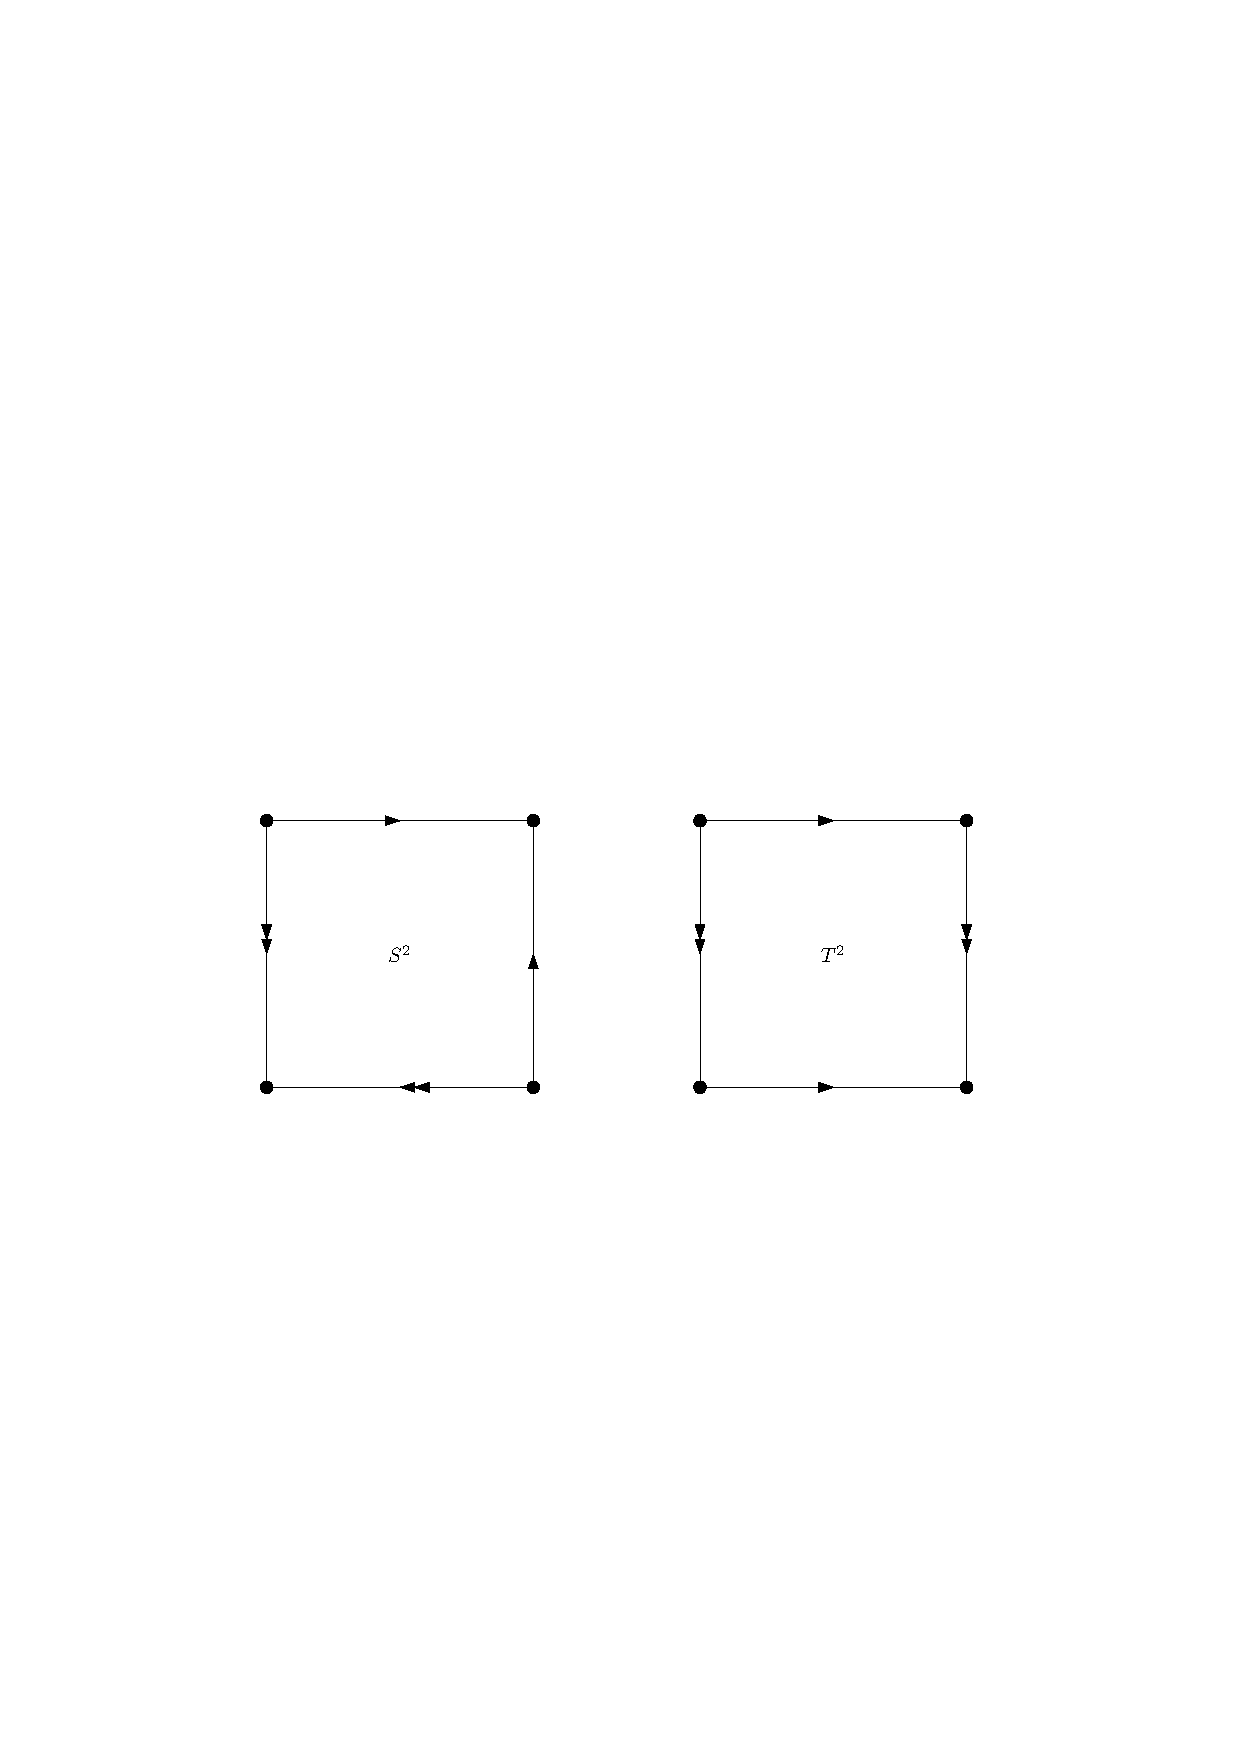
\includegraphics[width=0.7\linewidth]{square_representation}
	\caption{Represent $ S^2 $ and $ T^2 $ as quotient spaces of unit square} \label{fig:squarerepresentation}
\end{figure}
\begin{figure}
	\centering
	\includegraphics[width=0.7\linewidth]{"delete hole"}
	\caption{Puncture a hole in the square}
	\label{fig:delete-hole}
\end{figure}
\begin{sol}
	As Figure \ref{fig:squarerepresentation}, we represent $ S^2 $ and $ T^2 $ as quotient spaces of unit square. Then by counting different vertices and edges after gluing, we have
	\begin{align*}
		\chi(S^2)&=c_0-c_1+c_2=3-2+1=2\\ \chi(T^2)&=c_0-c_1+c_2=1-2+1=0.
	\end{align*}
	
	To calculate Euler characteristic of $ n $ disks punctured $ S^2 $ or $ T^2 $, we turn to consider punctured square, as Figure \ref{fig:delete-hole}. Add a regular $ n $-polygon in the center of square, connect each vertex of $ n $-polygon with all vertices of that square. Then replace vertex in the regular $ n $-polygon with an irregular $ 6 $-polygon for which we delete the interior part. And we color new generated vertices and edges in purples.
	
	Denote $ S_n^2 $ and $ T_n^2 $ corresponding $ n $-disks punctured $ S_n^2 $ and $ T_n^2 $. After identifying some vertices in square, we calculate
		\begin{align*}
	\chi(S^2_n)&=c_0'-c_1'+c_2'=(c_0+n(-1 + c_0 +2))-(c_1 +n(c_0 +2))+c_2\\&=(3+4n)-(2+5n)+1=2-n\\ 	\chi(T^2_n)&=c_0'-c_1'+c_2'=(c_0+n(-1 + c_0 +2))-(c_1 +n(c_0 +2))+c_2\\&=(1+4n)-(2+5n)+1=-n.
	\end{align*}
	 
\end{sol}

\begin{prop}
	La surface à bord $S_{C}$ est homéomorphe à $X \backslash\left(\mathring{D}_{1}^{2} \sqcup \mathring{D}_{2}^{2} \sqcup \cdots \sqcup \mathring{D}_{n}^{2}\right)$ où $X$ est l'une des surfaces $S^{2}$ ou $T^{2} .$ Peut-on déterminer laquelle en utilisant uniquement la caractéristique d'Euler?
\end{prop}
\begin{sol}
	No, we cannot because we have $ \chi(S_C) =-4= \chi(S^2_6)=\chi(T^2_4) $.
\end{sol}
\begin{prop}
	Révisez la notion de variété à bord. On remarque que $S_{C}$ et $C$ sont des variétés de dimension 2 à bord et que $\pi_{1}: S_{C} \rightarrow C$ est une application différentiable. Compter le nombre de composantes de bord de $S_{C}$ (i.e. le nombre de composantes connexes de $\partial S_{C}$). Répondre alors au point précédent.
\end{prop}
\begin{sol}
	To see that $ S_C $ has smooth boundary, we can enlarge the outer radius and reduce the value of $ \epsilon $ in $ C $ then the boundary of $ S_C $ can be seen as the  locally homeomorphism preimage of smooth circles hence smooth as well. $ \pi_{1}: S_C \rightarrow C $ is the restriction to a regular submanifold of a smooth map between two manifolds $  \mathbb{C}^2 $ and $ \mathbb{C} $ and hence smooth again.
	
	The preimage of a component in $ \partial C $ is connected in $ S_C $ since here we can topologically view this covering map as $ p: z \in S^1 \mapsto z^2 \in S^1 $ in complex plane. Therefore, there are four components in $ \partial S_C $ and for previous question we then know $ S_C $ is homeomorphic to $T^{2}_{4}:=T^{2} \backslash\left(\mathring{D}_{1}^{2} \sqcup \mathring{D}_{2}^{2} \sqcup \mathring{D}_{3}^{2} \sqcup \mathring{D}_{4}^{2}\right)$.
\end{sol}
\begin{prop}
	Si on considère $S_{C} \cup S^{0} \cup S^{1} \cup S^{2}$ alors il s'agit d'une variété de dimension 2 homéomorphe à une de la liste ci-dessus. Laquelle?
\end{prop}
\begin{sol}
	We have four homeomorphisms
	\begin{align*}
		\pi_{1}:& S_C \cong T^{2} \backslash\left(\mathring{D}_{1}^{2} \sqcup \mathring{D}_{2}^{2} \sqcup \mathring{D}_{3}^{2} \sqcup \mathring{D}_{4}^{2}\right) \\
		\pi_{2}:& S^i \cong D(i,\epsilon),\, \text{ where }i\in \{1,2,3\},		
	\end{align*}
	combine them we get $S_{C} \cup S^{0} \cup S^{1} \cup S^{2} \cong T^{2}_1:=T^{2} \backslash\mathring{D}_{1}^{2}. $
\end{sol}
\end{document}
